%%%%%%%%%%%%%%%%%%%%%%%%%%%%%%%%%%%%%%%%%
% Jacobs Landscape Poster
% LaTeX Template
% Version 1.0 (29/03/13)
%
% Created by:
% Computational Physics and Biophysics Group, Jacobs University
% https://teamwork.jacobs-university.de:8443/confluence/display/CoPandBiG/LaTeX+Poster
% 
% Further modified by:
% Nathaniel Johnston (nathaniel@njohnston.ca)
%
% This template has been downloaded from:
% http://www.LaTeXTemplates.com
%
% 
% Masaryk University presentation themes were downloaded from:
% https://www.overleaf.com/gallery/tagged/muni
%
% and ported into Jacobs Landscape Poster by:
% Jumaidil Awal (ideal1st.here@googlemail.com)
% 
% Jacobs Landscape Poster License:
% CC BY-NC-SA 3.0 (http://creativecommons.org/licenses/by-nc-sa/3.0/)
%
% Masaryk University's fibeamer theme license:
% Copyright 2015  Vít Novotný <witiko@mail.muni.cz>
% Faculty of Informatics, Masaryk University (Brno, Czech Republic)
% under Latex Project Public License
%
%%%%%%%%%%%%%%%%%%%%%%%%%%%%%%%%%%%%%%%%%

%----------------------------------------------------------------------------------------
%	PACKAGES AND OTHER DOCUMENT CONFIGURATIONS
%----------------------------------------------------------------------------------------

\documentclass[final]{beamer}

\usepackage{url}

\usepackage[maxbibnames=10]{biblatex}
\renewbibmacro{in:}{}
\addbibresource{refposter.bib}

\usepackage[scale=0.849]{beamerposter} % Use the beamerposter package for laying out the poster

%\usetheme{confposter} % Use the confposter theme supplied with this template
\usetheme[faculty=chemo]{fibeamer} % Uncomment to use Masaryk University's fibeamer theme instead.

%\setbeamercolor{block title}{fg=ngreen,bg=white} % Colors of the block titles
%\setbeamercolor{block body}{fg=black,bg=white} % Colors of the body of blocks
%\setbeamercolor{block alerted title}{fg=white,bg=ngreen} % Colors of the highlighted block titles
%\setbeamercolor{block alerted body}{fg=black,bg=dblue!10} % Colors of the body of highlighted blocks
% Many more colors are available for use in beamerthemeconfposter.sty

%-----------------------------------------------------------
% Define the column widths and overall poster size
% To set effective sepwid, onecolwid and twocolwid values, first choose how many columns you want and how much separation you want between columns
% In this template, the separation width chosen is 0.024 of the paper width and a 4-column layout
% onecolwid should therefore be (1-(# of columns+1)*sepwid)/# of columns e.g. (1-(4+1)*0.024)/4 = 0.22
% Set twocolwid to be (2*onecolwid)+sepwid = 0.464
% Set threecolwid to be (3*onecolwid)+2*sepwid = 0.708

\newlength{\sepwid}
\newlength{\onecolwid}
\newlength{\twocolwid}
\newlength{\threecolwid}
\newlength{\fourcolwid}
\setlength{\paperwidth}{49.35in} % A0 width: 46.8in
\setlength{\paperheight}{33.1in} % A0 height: 33.1in
\setlength{\sepwid}{0.018\paperwidth} % Separation width (white space) between columns
\setlength{\onecolwid}{0.31\paperwidth} % Width of one column
\setlength{\twocolwid}{0.451\paperwidth} % Width of two columns
\setlength{\threecolwid}{0.64\paperwidth} % Width of three columns
\setlength{\fourcolwid}{0.97\paperwidth} % Width of four columns
%\setlength{\topmargin}{-0.5in} % Reduce the top margin size
%-----------------------------------------------------------

% Theorems
\newtheorem{thm}{Theorem}[section]
%\newtheorem{proof}[thm]{Proof}
%\newtheorem{lemma}[thm]{Lemma}
\newtheorem{rem}[thm]{Remark}
\newtheorem{cor}[thm]{Corollary}
\newtheorem{ex}[thm]{Example}
\newtheorem{assu}[thm]{Assumption}
\newtheorem{alg}[thm]{Algorithm}
\newtheorem{defn}[thm]{Definition}
\newtheorem{app1}[thm]{Image Processing}
\newtheorem{app2}[thm]{Text Mining}
\newcommand{\real}{\mathbb{R}}

\DeclareMathOperator{\rank}{rank}
\DeclareMathOperator{\bc}{bc}


\usepackage{caption}
\captionsetup[figure]{labelformat=simple}

\usepackage{mathtools}
\DeclarePairedDelimiterX{\norm}[1]{\lVert}{\rVert}{#1}

\usepackage{graphicx}  % Required for including images

\usepackage{booktabs} % Top and bottom rules for tables

\usepackage{comment}
%----------------------------------------------------------------------------------------
%	TITLE SECTION 
%----------------------------------------------------------------------------------------

\title{The Why and How of Nonnegative Matrix Factorization} % Poster title

\author{LINMA2380 --- Group 2 --- Aurélie de Borman, Jennifer Leclipteur, Gilles Peiffer, and Minh-Phuong Tran} % Author(s)

\institute{École Polytechnique de Louvain, UCLouvain} % Institution(s)

%----------------------------------------------------------------------------------------

\begin{document}
\addtobeamertemplate{block end}{}{\vspace*{1ex}} % White space under blocks
%\addtobeamertemplate{block example end}{}{\vspace*{2ex}} % White space under example blocks
\addtobeamertemplate{block example end}{}{\vspace*{1ex}}
\addtobeamertemplate{block alerted end}{}{\vspace*{1ex}} % White space under highlighted (alert) blocks

\setlength{\belowcaptionskip}{2ex} % White space under figures
\setlength\belowdisplayshortskip{2ex} % White space under equations
%\begin{darkframes} % Uncomment for dark theme, don't forget to \end{darkframes}
\begin{frame} % The whole poster is enclosed in one beamer frame

%==========================Begin Head===============================

  \begin{columns}[t]
   \begin{column}{\linewidth}
    \vskip0.5cm
    \centering
    \usebeamercolor{title in headline}{\color{fg}\Huge{\textbf{\inserttitle}}\\[0.3ex]}
    \usebeamercolor{author in headline}{\color{fg}\large{\insertauthor}\\[0.3ex]}
    %\usebeamercolor{institute in headline}{\color{fg}\large{\insertinstitute}\\[1ex]}
   \end{column}
  \end{columns}
 \vspace{2cm}

%==========================End Head===============================

\begin{columns}[t] % The whole poster consists of three major columns, the second of which is split into two columns twice - the [t] option aligns each column's content to the top
\begin{column}{\sepwid}
\end{column} % Empty spacer column
\begin{column}{\threecolwid}
%----------------------------------------------------------------------------------------
%	Introduction and Motivation
%----------------------------------------------------------------------------------------

\begin{alertblock}{In a Few Words}
\normalsize
\textbf{Nonnegative matrix factorization} (NMF) is a powerful tool for the analysis of \textbf{high-dimensional} data as it automatically extracts \textbf{sparse} and \textbf{meaningful} features from a set of \textbf{nonnegative} vectors.
\end{alertblock}

%----------------------------------------------------------------------------------------
%	Nonnegative Matrix Factorization: definition and properties (sparse, meaningful features)
%----------------------------------------------------------------------------------------

\begin{exampleblock}{Nonnegative Matrix Factorization: Definition and Properties}
The goal of \textbf{NMF} is to decompose a given nonnegative data matrix $X$ as $X \approx W H$ where $W$ and $H$ are also nonnegative matrices.

NMF is a linear dimensionality reduction (LDR) tool. As a reminder, a LDR method computes a set of $r < \min(p,n)$ basis elements $w_k \in \real^p$ for $1 \leqslant k \leqslant r$ to approximate a set of data points $x_j \in \real^{p}$ for $1 \leqslant j \leqslant n$ such that for all $j$ we have $x_j \approx \sum_{k = 1}^{r} w_{k} h_{j}(k)$, for some weights $h_j\in \real^r$.

%LDR is equivalent to low-rank matrix approximation where: $X \approx W H$ where \\
The data matrix $X$ is approximated by a low-rank product of matrices $WH$, with:
     \begin{itemize}
     \item $X \in \real^{p \times n}$: $X(:,j) = x_j$ for $1 \leqslant j \leqslant n$. Each column of the matrix $X$ is a data point.
     \item $W \in \real^{p \times r}$: $W(:,k) = w_k$ for $1 \leqslant k \leqslant r$. Each column of the matrix $W$ is a basis element.
     \item $H \in \real^{r \times n}$: $H(:,j) = h_j$ for $1 \leqslant j \leqslant n$. Each column of the matrix \(H\) gives the coordinates of a data point \(X(:,j)\) in the basis associated to \(W\).
     \end{itemize}
\end{exampleblock}



%----------------------------------------------------------------------------------------
%	Applications
%----------------------------------------------------------------------------------------

\begin{exampleblock}{Applications}
\vspace{-0.8cm}
\begin{columns}[t]
\begin{column}{\onecolwid}

The following applications rely heavily on the use of nonnegative matrix factorization.
Note that this list is not exhaustive by any means.

\vspace{0.3cm}

\begin{block}{Image Processing}
\textbf{Goal}: facial feature extraction.

The \textbf{data matrix} $X\in\real^{p\times n}_+$ carries information about $n$ face images. Each image has $p$ pixels and therefore each column of $X$ represents an image of a face.
This means $X(i, j)$ represents the gray level of the $i$-th pixel in the $j$-th face.

The \textbf{nonnegative matrix factorization} for this problem can be interpreted as follows:
\begin{itemize}
    \item Each column of the matrix $W$ represents a facial feature.
    \item $H(k, j)$ represents the importance of the $k$-th feature in the $j$-th face.
\end{itemize}
\begin{figure}
    \centering
    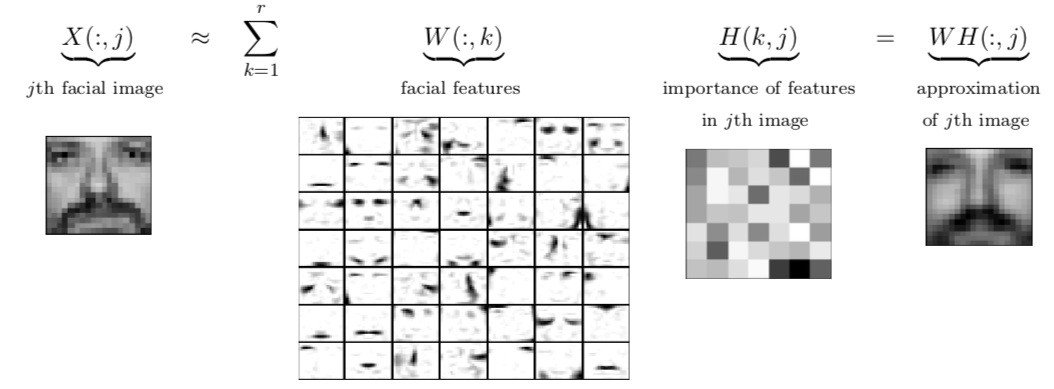
\includegraphics{../images/NMF_app1.png}
\end{figure}
\end{block}
\end{column}
\begin{column}{\onecolwid}

\begin{block}{Hyperspectral Unmixing}
\textbf{Goal}: identify the constitutive materials present in an image and classify the pixels according to the abundance of each constitutive material.

The \textbf{data matrix} $X\in\real^{n\times p}_+$ encodes the spectral signatures of the pixels in a scene being imaged.

The \textit{spectral signature} of a pixel is the fraction of incident light being reflected by that pixel at different wavelengths.
This means \(X(i, j)\) represents the spectral signature of the $j$-th pixel at the $i$-th considered wavelength.

The \textbf{nonnegative matrix factorization} for this problem can be interpreted as follows:

\begin{itemize}
    \item Each column of the matrix $W$ represents the spectral signature of a material (such as road, grass,\dots).
    \item $H(k, j)$ represents the abundance of the $k$-th material in the $j$-th pixel.
\end{itemize}
\begin{figure}
    \centering
    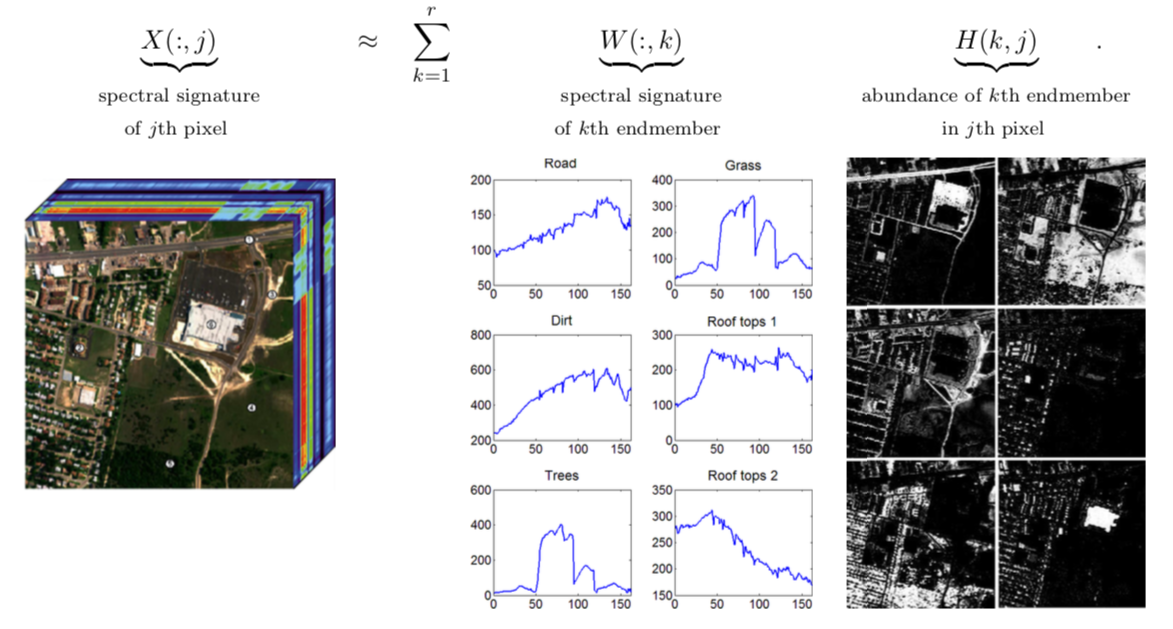
\includegraphics[width=0.8\linewidth]{../images/NMF_app3.png}
\end{figure}
\end{block}
\end{column}
\end{columns}
\begin{block}{Text Mining}
\textbf{Goal}: topic recovery and document classification.

The \textbf{data matrix} $X\in\real^{n\times n}_+$ encodes the frequency of some words in a list of documents.
This means $X(i, j)$ represents the number of times the $i$-th word appears in the $j$-th document.

The \textbf{nonnegative matrix factorization} for this problem can be interpreted as follows:

\begin{itemize}
    \item Each column of the matrix $W$ represents a topic.
    \item $H(k, j)$ represents the importance of the $k$-th topic in the $j$-th document.
\end{itemize}
\begin{figure}
    \centering
    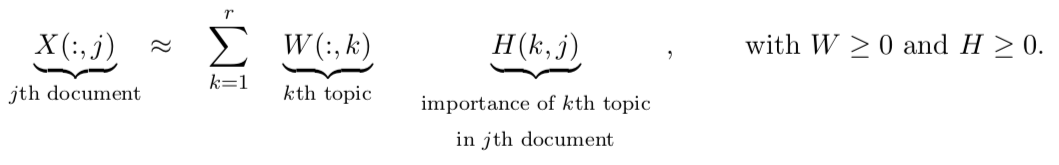
\includegraphics{../images/NMF_app2.png}
\end{figure}
\end{block}
\end{exampleblock}
\begin{exampleblock}{References}
\nocite{NMF}
\nocite{biclique}
\printbibliography
\end{exampleblock}
\end{column}
\begin{column}{\sepwid}
\end{column} % Empty spacer column
\begin{column}{\onecolwid} % The third column


%----------------------------------------------------------------------------------------
%	Links to other problems
%----------------------------------------------------------------------------------------
\begin{exampleblock}{Problem Formalization and Algorithmic Difficulties}
\vspace{0.4cm}
\begin{block}{Optimization Problem}
We want to solve \(\displaystyle \min_{W \in \real^{p \times r}, H \in \real^{r \times n}} \norm{X - WH}^2_{\textnormal{F}}\), such that \(W \geqslant 0\), \(H \geqslant 0\).
Our use of the Frobenius norm implies the assumption that the noise is Gaussian.
This is not always the best choice; in practice, depending on the application, other choices are possible too, such as:
\begin{itemize}
    \item the Kullback--Leibler divergence, used in text mining;
    \item the Itakura--Saito distance, used in music analysis;
    \item the \(\ell_1\) norm used to improve robustness against outliers; etc.
\end{itemize}
\end{block}
\begin{block}{Algorithmic Difficulties}
NMF is not a trivial task:
\begin{itemize}
    \item NMF is \textbf{NP-hard} because of the nonnegativity constraints.
    In the unconstrained case, the SVD can be used.
    In practice, assumptions and heuristics allow us to solve the problem fairly efficiently.
    \item NMF is \textbf{ill-posed}: if \((W, H)\) is an NMF of \(X\), then so is \((W', H') = (WQ, Q^{-1}H)\), where \(WQ \geqslant 0\), \(Q^{-1}H \geqslant 0\).
    This can be solved by
    \begin{itemize}
        \item using \textbf{priors} for \(W\) and \(H\), such as sparsity;
        \item adding \textbf{regularization} terms.
    \end{itemize}
    Finding application-specific solutions is an active area of research.
\end{itemize}
\end{block}
\end{exampleblock}

\begin{exampleblock}{Connections to Other Problems}
Nonnegative matrix factorization is closely related to many other problems; the following (non-exhaustive) list of \textbf{connections} between NMF and other mathematical problems is interesting to consider.

\begin{defn}[Nonnegative Rank]
Given $X \in \real_+^{p\times n}$, the nonnegative rank of \(X\), denoted $\rank_+(X)$, is the minimum $r$ such that there exists $W \in \real_+^{p\times r}, H \in \real_+^{r\times n}$ with $X = WH$.
\end{defn}

%Intuitively, the columns of X can be seen as vectors that we want to generate from a basis formed by the columns of W. We want our basis to have as few vectors as possible.
%~\\
%~\\
\begin{block}{Graph Theory: Bipartite Dimension}
Finding the \textbf{bipartite dimension} of a graph gives a lower bound for the nonnegative rank of the matrix inducing that graph. Indeed, let $G(X) = (V_1 \cup V_2, E)$ be the bipartite graph induced by \(X\) (i.e. $(i,j)\in E \iff X_{ij}\neq 0$). 
    
The bipartite dimension (also called ``minimum biclique cover'') $\bc(G(X))$ is the minimum number of bicliques needed to cover all edges in \(E\).

The formula for the rectangle covering bound is then given by \(\bc(G(X)) \leqslant \rank_+(X)\).
\end{block}

\begin{block}{Linear Optimization: Extended Formulation}
The \textbf{extended formulation} of a polytope \(P\) is composed of a higher dimensional polytope \(Q\) and a linear projection $\pi$ such that $\pi(Q) = P$.
\[
\begin{array}{l@{\quad}rcl}
\max \quad c^\top x&&& \\
\textnormal{s.t.} & Ax & \leqslant & b\\
& x \in \real^n & \geqslant & 0
\end{array}
\tag{\textnormal{LP}}
\]
Finding the minimum size of an extended formulation of the polytope defined by the constraints amounts to computing the nonnegative rank of the slack matrix with elements $X(i,j) = b_i-A_iv_j$ with $v_j$ the $j$-th vertex of \(P\) and $\{x\in \real^n \mid b_i-A_ix\geqslant 0\}$ its $i$-th facet.
Finding an extended formulation is interesting in that it allows to solve problem~(LP) in polynomial time.
\end{block}

\end{exampleblock}

\begin{alertblock}{Conclusion}
Nonnegative matrix factorization not only generates meaningful features, but also has many applications in various domains. Although there are theoretical difficulties one has to deal with when using this linear dimensionality reduction technique, such as its NP-hardness and ill-posedness, mathematical research has come a long way in finding creative solutions to many of these issues.
Additionally, it is intimately related to many other domains of mathematics.
\end{alertblock}

\end{column}
\begin{column}{\sepwid}
\end{column} % Empty spacer column
\end{columns} % End of all the columns in the poster
\begin{columns}[t]
\begin{column}{\sepwid}
\end{column} % Empty spacer column
\begin{column}{\fourcolwid}
%----------------------------------------------------------------------------------------
%	References
%----------------------------------------------------------------------------------------
%\begin{alertblock}{References}
%\nocite{biclique}
%\nocite{NMF}
%\printbibliography
%\end{alertblock}
\end{column}
\end{columns}
\end{frame} % End of the enclosing frame
%\end{darkframes} % Uncomment for dark theme
\end{document}
